\documentclass[11pt,paper=letter]{scrartcl}
\usepackage[alttitle]{cjquines}

\begin{document}

\title{What is $n$ choose 2?}
\author{Carl Joshua Quines}
\date{July 14, 2020}

\maketitle

All of the problems today have the same theme: what is $\binom{n}{2}$? The answer to that is that it represents pairs of the $n$ things. Thinking about the meaning of this will usually give a solution, either directly, with Jensen, double counting, an expected value argument, parity, or something else.

\subsubsection*{Warmup}

\begin{enumerate}

\item In a graph, the average degree of the vertices is $4.5$. Prove there is a vertex with degree at most $4$. Prove there is a vertex with degree at least $5$.

\item (Handshake) Prove that, in a graph, the sum of the degrees of the vertices is even.

\item (USA TST 2005) Let $n$ be an integer greater than $1$. For a positive integer $m$, let $S_m = \{1, 2, \ldots, mn\}$. Suppose there exists a $2n$-element set $T$ such that
\begin{enumerate}
  \item each element of $T$ is an $m$-element subset of $S_m$,
  \item each pair of elements of $T$ shares at most one common element, and
  \item each element of $S_m$ is contained in exactly two elements of $T$.
\end{enumerate}
Determine the maximum possible value of $m$ in terms of $n$.

\textbf{Hint:} What is $\binom{2n}{2}$?

\textbf{Solution:} We know $\binom{2n}{2}$ counts the pairs of sets in $T$, but what does that mean? The problem says that any pair of sets shares at most one common element. So these pairs produce at most $\binom{2n}{2}$ elements.

Can any of these elements be the same? Well, if they were, that would mean that three or more sets shared a common element. But this contradicts the third condition. So that means that all of these $\binom{2n}{2}$ elements are different.

Since there are only $mn$ elements, we get $mn \le \binom{2n}{2}$, so $m \le 2n - 1$. To show $m = 2n - 1$ possible, consider $2n$ lines in the plane, no two of which are parallel and no three of which are concurrent.

\end{enumerate}

\subsubsection*{Examples}

\begin{enumerate}

\item (Iran 2010) There are $n$ points in the plane such that no three of them are collinear. Prove that the number of triangles whose vertices are chosen from these $n$ points and whose area is $1$ is not greater than $\frac{2}{3}(n^2 - n)$.

\textbf{Hint.} What is $\binom{n}{2}$?

\textbf{Solution.} We want to show there can't be too many triangles with area $1$, so we want to limit the number of triangles in some way. In total, we know there are $\binom{n}{3}$ triangles, because you take any three points, and they determine a triangle. In other words, if you fix three points, then you can make only one triangle after them. This is too large, of course, since we only need to count triangles with area $1$.

So instead, let's look at $\binom{n}{2}$, which we know represents pairs of points. Previously, we know that given three points, there was only one triangle. What about given two points? There are $n - 2$ choices for the third point, so there would be $n - 2$ triangles. But can all of these triangles have area $1$?

\begin{center}
  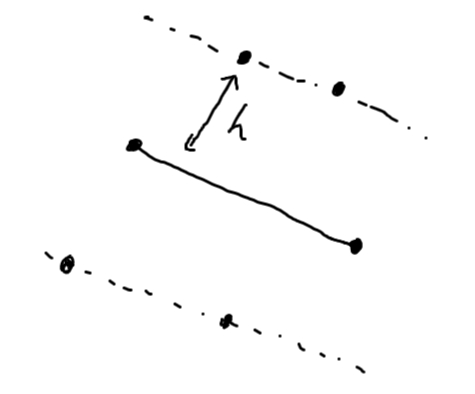
\includegraphics[height=2in]{198.jpg}
\end{center}

We can find the area of the triangle by treating these two chosen points as the base. Then there's only one choice for the height. So the third point must lie in one of two lines. Can we have all $n - 2$ points lying on these two lines? We can't---because no three points are collinear. Each of these two lines can have at most $2$ points on them. So given two points, there are at most $4$ triangles of area $1$ that contain both.

Now, we'll add up the $4$ triangles for each of the $\binom{n}{2}$ pairs of points. This gives us at most $4\binom{n}{2}$ triangles. Except we've counted each triangle multiple times. We've counted a triangle thrice, once for each pair of points. So we should divide $4\binom{n}{2}$ by $3$. The number of triangles with area $1$ is now at most $\frac{4}{3}\binom{n}{2}$, which is $\frac{2}{3}(n^2 - n)$.

\textbf{Remark.} This is what a double counting argument should feel like. Very generally, there's some \textit{small counting}, or \textit{local counting} going on. By taking the sum of these small counts, we can relate it to some \textit{big count}, or \textit{global count}. In this problem, the small count was the triangles formed by a pair of points, and the big count was the number of triangles in general. We'll make this clearer later.

\item (IMO 1987) Let $n$ and $k$ be positive integers and let $S$ be a set of $n$ points in the plane such that,
\begin{enumerate}
  \item no three points of $S$ are collinear, and
  \item for every point $P$ in $S$, there are at least $k$ points in $S$ equidistant from $P$.
\end{enumerate}
Prove that $k < \frac{1}{2} + \sqrt{2n}$.

\textbf{Hint:} What is $\binom{k}{2}$?

\textbf{Solution:} For a given point, the number of pairs of points equidistant to it are at least $\binom{k}{2}$. Sum over each of the $n$ points to get $n\binom{k}{2}$. Like the previous solution, we've counted some pairs of points multiple times. Note that when we count a pair of points, it means we have a point that's equidistant to both.

\begin{center}
  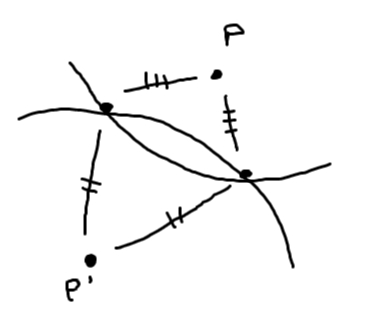
\includegraphics[height=2in]{199.jpg}
\end{center}

So that means the point that counts that pair must lie on the perpendicular bisector. Since no three points are collinear, a pair of points is counted at most twice. This gives us $n\binom{k}{2} \le 2\binom{n}{2}$, which rearranges to the answer.

\textbf{Remark 1.} The small counting and big counting is clearer in this example. The small count is the number of pairs of points equidistant to a given point. By adding all of these together, we've related it to the big count, which is the number of pairs of points in general. The theme is ``sum of small pairs relates to total pairs'' will appear a lot in this set.

\textbf{Remark 2.} Let's be a bit more specific about that inequality in the end. What each pair of points $a$ and $b$ counts, precisely, is a \textit{triplet} of points, $a$, $b$ and $c$, such that $c$ is equidistant to $a$ and $b$. Let's say there are $T$ such triplets of points.

The first part of our solution shows $T \ge n\binom{k}{2}$: for each point, we can find at least $\binom{k}{2}$ triplets. The second part of our solution shows that $T \le 2\binom{n}{2}$: each pair of points gives at most two triplets. It's combining these that gives the inequality.

If we wanted to, we can write the previous solution in this way as well. The triplets you're counting are three points, $a$, $b$, and $c$, such that $c$ has distance $1$ from the line formed by $a$ and $b$. The first part of the solution showed $T \le 4\binom{n}{2}$, because each pair of points gives at most $4$ triplets. The second part of the solution shows that $T$ is at least $3$ times the number of triangles, because each triangle of area $1$ gives three triplets.

\item (Kinda NOI.PH 2017) In a party with $n$ people, there are at least $\frac{1}{4}(n + 1)^2$ pairs of people who are friends with each other. Call a triplet of people $A$, $B$, and $C$ a \textit{mutual friendzone} if $A$ is friends with $B$, and $B$ is friends with $C$. Prove that there are at least $\frac{1}{4}(n^3 - n)$ mutual friendzones.

\textbf{Hint:} Let the degree of someone be $d$. What is $\binom{d}{2}$?

\textbf{Solution:} Consider the graph with people as vertices, and edges as friends. Let's say the degree of a vertex is $d$. Then $\binom{d}{2}$ counts pairs of that vertex's neighbors. If that vertex is $B$, for example, then this counts two of its neighbors $A$ and $C$. So $\binom{d}{2}$ counts the number of mutual friendzones ``centered'' at a given vertex.

Let the degrees of each vertex be $d_1, \ldots d_n$. Then the number of mutual friendzones is \[
  \binom{d_1}{2} + \cdots + \binom{d_n}{2}.
\]
So far, we've done the small counts and taken their sum. We now need to find a lower bound. Here comes the trick: we'll use Jensen. Because the function $\binom{n}{2}$ is convex, we can do \[
  \binom{d_1}{2} + \cdots + \binom{d_n}{2} \ge n\binom{\left(d_1 + \cdots + d_n\right)/n}{2}.
\]
This is what Jensen tells us: the sum is minimized when each of the $d_i$ is equal to their average. But we know what $d_1 + \cdots + d_n$ is. By the handshake lemma, it's just twice the number of edges, so it's $\frac{1}{2}(n + 1)^2$. Thus:
\[
  n\binom{\left(d_1 + \cdots + d_n\right)/n}{2} = n\frac{(n + 1)^2/(2n)}{2} > n\binom{(n + 1)/2}{2} = \frac{n^3 - n}{4}.
\]

\textbf{Remark:} The trick of using Jensen to combine the small counts is going to appear several times in this set too. 

\end{enumerate}

\subsubsection*{Problems}

\begin{enumerate}

\item (IMO 1998) In a competition, there are $a$ contestants and $b$ judges, where $b \ge 3$ is an odd integer. Each judge rates each contestant as either ``pass'' or ``fail''. Suppose $k$ is a number such that for any two judges, their ratings coincide for at most $k$ contestants. Prove that \[
  \frac{k}{a} \ge \frac{b-1}{2b}.
\] \hints{\ref{h:1} \ref{h:2}}

\item A graph is \textit{squarefree} if it does not contain four points in a cycle. Prove that a squarefree graph with $n$ vertices has at most $\frac{n}{4}\left(1 + \sqrt{4n - 3}\right)$ edges. \hints{\ref{h:3} \ref{h:4}}

\item (ISL 2004) There are $10001$ students at an university. Some students join together to form several clubs (a student may belong to different clubs). Some clubs join together to form several societies (a club may belong to different societies). There are a total of $k$ societies. Suppose that the following conditions hold:
\begin{enumerate}
  \item Each pair of students are in exactly one club together.
  \item For each student and each society, the student is in exactly one club of the society.
  \item Each club has an odd number of students. In addition, a club with $2m+1$ students ($m$ is a positive integer) is
in exactly $m$ societies.
\end{enumerate}
Find all possible values of $k$. \hints{\ref{h:7} \ref{h:8}}

\item (Canada 2006) In a tournament, each pair among the $2n + 1$ participants play against each other, and there are no ties. Call a triple of people $A$, $B$, and $C$ a \textit{non-cyclic triplet} if $A$ won against $B$, $A$ won against $C$, and $B$ won against $C$. What is the minimum number of non-cyclic triplets?  \hint{\ref{h:9}}

\item (Iran 2010) A school has $n$ students and some classes. Each student can participate in any number of classes. Every class has at least two students participating. If two different classes have at least two common students, then the number of the students are distinct. Prove that the number of classes is at most $\left(n-1\right)^2$.  \hint{\ref{h:10}}

\item Let $a_1, \ldots, a_n$ be integers. Show that $\displaystyle \prod_{1 \le i < j \le n} (a_j - a_i)$ is divisible by $\displaystyle \prod_{1 \le i < j \le n} (j - i)$. \hints{\ref{h:5} \ref{h:6}}

\item (IMO 2015) We say that a finite set $\mathcal{S}$ of points in the plane is \textit{balanced} if, for any two different points $A$ and $B$ in $\mathcal{S}$, there is a point $C$ in $\mathcal{S}$ such that $AC = BC$. We say that $\mathcal{S}$ is \textit{center-free} if, for any three different points $A$, $B$ and $C$ in $\mathcal{S}$, there are no points $P$ in $\mathcal{S}$ such that $PA = PB = PC$.

\begin{enumerate}
  \item Show that for all integers $n \ge 3$, there exists a balanced set consisting of $n$ points.

  \item Determine all integers $n \ge 3$ for which there exists a balanced center-free set consisting of $n$ points. \hints{\ref{h:11} \ref{h:12}}
\end{enumerate}

\item (ISL 2016) Let $n \ge 5$ be a positive integer such that $\gcd(n, 6) = 1$. We color the vertices of a regular $n$-gon either red, blue, or black, such that every color is used on an odd number of vertices. Prove that there exists an isosceles triangle with vertices of all different colors. \hints{\ref{h:13} \ref{h:14}}

\end{enumerate}

\subsubsection*{Hints}

\begin{enumerate}
\item \label{h:5} To prove $a \mid b$, prove $\nu_p(a) \le \nu_p(b)$. (Here, for prime $p$, $\nu_p(a) = k$ if $p^k \mid a$ but $p^k \nmid a$.)
\item \label{h:8} Rewrite $\binom{2m + 1}{2} = m(2m + 1)$.
\item \label{h:11} For (b): what is $\binom{n}{2}$?
\item \label{h:13} Let $a$ be the number of red vertices. What is $\binom{a}{2}$?
\item \label{h:6} Let $k_1$ be the number of $a_1, \ldots, a_n$ that are $1$ modulo $p$. What is $\binom{k_1}{2}$?
\item \label{h:4} How does $\sum \binom{d}{2}$ relate to $\binom{n}{2}$?
\item \label{h:7} Suppose a club has $2m + 1$ members. What is $\binom{2m + 1}{2}$?
\item \label{h:1} What is $\binom{b}{2}$?
\item \label{h:9} Suppose person $i$ won $w_i$ times. What is $\binom{w_i}{2}$?
\item \label{h:14} How does $\binom{a}{2} + \binom{b}{2} + \binom{c}{2}$ relate to $\binom{n}{2}$?
\item \label{h:12} On average, how many times is a point counted by $\binom{n}{2}$?
\item \label{h:3} Suppose a vertex has degree $d$. What is $\binom{d}{2}$?
\item \label{h:10} For a class with $k$ people, what is $\binom{k}{2}$?
\item \label{h:2} For a given contestant, let's say that $x$ judges rated pass, and $b - x$ rated fail.
\end{enumerate}

\subsubsection*{Sketches}

\begin{enumerate}

\item The number of coinciding ratings over all judges is at most $k\binom{b}{2}$. Now take a given contestant, consider how each of the $b$ judges rate them. If $x$ rate them pass, this produces $\binom{x}{2} + \binom{b-x}{2} \ge \binom{(b-1)/2}{2} + \binom{(b + 1)/2}{2}$ coinciding ratings, by Jensen. Thus $a\left(\binom{(b-1)/2}{2} + \binom{(b + 1)/2}{2}\right) \le k\binom{b}{2}$, giving the result.

\item For a vertex with degree $d$, $\binom{d}{2}$ counts pairs of vertices. Sum over all vertices. Each pair of vertices is counted at most once; if it was counted twice it wouldn't be squarefree. So $\sum \binom{d}{2} \le \binom{n}{2}$, and using Jensen's gives the bound.

\item For a given club, $\binom{2m + 1}{2}$ counts the pairs of students in that club. Each pair is counted exactly once, so summing over all clubs, it must be $\binom{10001}{2}$. Also, note $\binom{2m + 1}{2} = m(2m + 1)$, which represents $2m + 1$ students, each a member of $m$ societies. Summing over all clubs should give $10001k$, the number of students and the number of societies they are each in. Then construct.

\item If person $i$ won $w_i$ times, $\binom{w_i}{2}$ is the number of non-cyclic triplets with that person as $A$. By Jensen there are at least $(2n + 1)\binom{n}{2}$ non-cyclic triplets. Construction left to reader.

\item For a class with $k$ people, $\binom{k}{2}$ counts pairs of students. Sum over all classes with $k$ students. Each pair of students is counted at most once, so there are at most $\binom{n}{2}/\binom{k}{2}$ classes with $k$ students. Sum over $k$.

\item Let $k_i$ be the number of $a_1, \ldots, a_n$ that are $i$ modulo $p$. The sum $\binom{k_0}{2} + \cdots + \binom{k_{p-1}}{2}$ is the exponent of $p$ in the numerator. By Jensen, this is minimized when $k_0, \ldots, k_{p-1}$ are as they are with $1, 2, \ldots, n$. This needs a bit more care to work out when, say, $p^2$ happens to divide the difference.

\item For (a), take a bunch of circles around a circle with center at $P$. For (b), it's the odd numbers: for the construction, take a regular $n$-gon.

To show even $n$ is impossible, note that the total number of $C$s is $\binom{n}{2}$. On average a point is the $C$ of a triplet $\frac{1}{n}\binom{n}{2} = \frac{n-1}{2}$ times. If $n$ is even, some point has to be $C$ an odd number of times, so it's not center-free.

\item Suppose there are no such triangles. Call an isosceles triangle with vertices all the same color \textit{monochromatic}. Then $\binom{a}{2} + \binom{b}{2} + \binom{c}{2}$ counts monochromatic triangles thrice, and other isosceles triangles once. Also, $\binom{n}{2}$ is the total number of isosceles triangles. Their difference is twice the number of monochromatic triangles, but for this $n$ it can't be even.

\end{enumerate}

\subsubsection*{Bonus}

\begin{enumerate}

\item In a tournament, each pair among the $n$ participants play against each other, and there are no ties. Let $w_i$ be the the number of times the $i$th person wins, and $l_i$ the number of times they lose. Show that the sum of $\binom{w_i}{2}$s is the same as the sum of $\binom{l_i}{2}$s.

% sketch: they're both number of non-cyclic triplets

% \item (Hong Kong 2007) In a school there are $2007$ girls and $2007$ boys. Each student joins no more than $100$ clubs in the school. It is known that any two students of opposite genders have joined at least one common club. Show that there is a club with at least $11$ boys and $11$ girls.

% \textbf{Sketch:} There are at least $2007^2$ pairs of boys and girls with a common club. Suppose otherwise. The clubs with at most $10$ boys contribute to this by at most $100 \cdot 10 \cdot 2007$, and similarly with girls, contradiction.

\item (USAMO 1995) Suppose that in a certain society, each pair of persons can be classified as either \textit{amicable} or \textit{hostile}. We shall say that each member of an amicable pair is a \textit{friend} of the other, and each member of a \textit{hostile} pair is a foe of the other. Suppose that the society has $n$ persons and $q$ amicable pairs, and that for every set of three persons, at least one pair is hostile. Prove that there is at least one member of the society whose foes include $q(1 - 4q/n^2)$ or fewer amicable pairs.

% \textbf{Sketch:} Consider the graph on friends. For a vertex $v$ with degree $d$, what are the edges that \textit{don't} connect two of its foes? There are $d$ edges connecting $v$ to its neighbors. There are no edges connecting two neighbors. If the neighbors of $v$ have degrees $d_1, \ldots, d_d$, then there are $d_1 + \cdots + d_d - d$ edges connecting one of $v$'s neighbors to something that isn't $v$. Add over all vertices and use Jensen to get $\sum d^2 \ge 4q^2/n$. So some vertex has at least $4q^2/n^2$ edges that don't connect two of its foes, leaving at most $q - 4q^2/n^2$ edges that do.
 
\end{enumerate}

\subsubsection*{References}

Problems were mostly lifted from Kraknova's \href{https://euclid.ucc.ie/mathenr/IMOTraining/2010 Summer Camp - Victoria Krakovna - Double Counting.pdf}{Double Counting} handout, and chapter 6 of Sriram's \href{https://euclid.ucc.ie/mathenr/IMOTraining/CombinatoricsChapter6 Aug 2014.pdf}{Olympiad Combinatorics}.

\end{document}
